\documentclass[11pt,a4paper]{article}
\usepackage[utf8]{inputenc}
\usepackage{report-style}
\usepackage{hyperref}
\usepackage{graphicx}



\begin{document}



\tableofcontents

\newpage

\section{Introduction}

In this Machine Learning and Data Mining project, we have developed a customer churn prediction model for a bank dataset. The model aims to predict whether new customers are likely to stay or leave the bank, addressing the critical challenge of customer churn. By accurately predicting churn, the bank can take proactive measures to retain customers and improve service quality. The project follows a well-structured approach, starting with data loading and exploration, followed by data preprocessing to ensure data quality. We analyze churn counts and visualize customer behavior to identify potential patterns related to churn. Using machine learning techniques, including the Random Forest Classifier, we evaluate the model's performance and present key metrics such as ROC curve, AUC score, and confusion matrix, providing valuable insights for customer retention strategies.

The project aims to build a customer churn prediction model for a bank's new customers, forecasting whether they will stay or leave. This model is crucial as it enables the bank to take proactive actions to retain customers, reduce churn rates, and optimize marketing and operational strategies. By leveraging data-driven insights, the bank can enhance customer satisfaction and strengthen its competitive position in the market, leading to improved business performance and long-term customer loyalty.

\subsection{Related work}

Guo-en and Wei-dong (2008) focused on building a customer churn prediction model using SVM in the telecommunication industry. They compared this method with other techniques such as DT, artificial neural networks, naïve Bayesian (NB) and logistic regression. The results proved SVM to be a simple classification method of high capability yet good precision. \cite{article}

Nie et al. (2011) built a customer churn prediction model by using logistic regression and DT-based techniques within the context of the banking industry. \cite{journals/eswa/NieRZTS11}

In their study, Lin et al.(2012) presented new-features-based logistic regression (LR), linear classifier (LC), NB, DT, MLP neural networks, and SVM. In their experiments, each technique produced a different output. Data mining by evolutionary learning (DMEL) could show the reason or probability of a churning phenomenon; DT, however, could only show the reason. LR, NB, and MLP could provide probabilities of different customer behaviors. LC and SVM could distinguish between a churner and a non-churner. \cite{LIN20118}

Keramati et al. (2014) not only presented different approaches to data mining and classification methods such as DT, neural networks, SVM, and k-nearest neighbors, but also had the performances of these approaches compared. They analyzed, as a case study, data from an Iranian mobile company. \cite{NIE201115273}



\section{Data Preparation}

Data Preparation is a crucial stage in the customer churn prediction project, where we carefully clean, preprocess, and organize the raw bank dataset to make it suitable for further analysis and model building. This phase involves several key steps: 

\subsection{Loading and Exploration}

\begin{figure}[H]
    \centering
    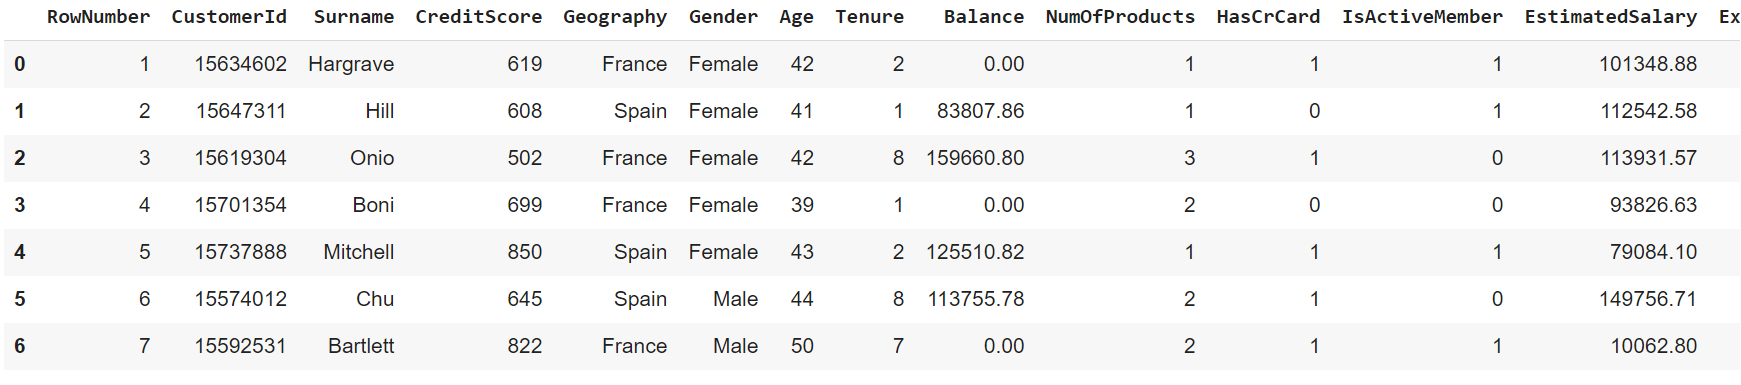
\includegraphics[width=1\textwidth]{Load the data.png}
    \caption{Dataset}
    \label{fig:enter-label}
\end{figure}

We start by loading the dataset into our data analysis environment. This allows us to understand the structure of the data, including the number of rows and columns, and the types of variables present. Exploring the dataset helps us gain initial insights into the data's characteristics and potential challenges we may encounter during data preparation.


\subsection{Data Preprocessing}

Data preprocessing is an essential step in data preparation that addresses various data quality issues. This includes:

\begin{enumerate}
    \item Handling Missing or Null Values: We identify any missing or null values in the dataset and decide on appropriate strategies to handle them. Depending on the extent of missing data and the nature of the variables, we may choose to impute missing values using methods like mean, median, mode, or advanced imputation techniques.
    \item Dealing with Categorical Variables: Since many machine learning algorithms require numerical inputs, we convert categorical variables into numerical representations. To avoid the dummy variable trap, we may use techniques like one-hot encoding or label encoding.
    \item Feature Scaling: To ensure fair treatment of different features during model training, we standardize the numerical features, bringing them to a similar scale.
    

\begin{figure}[H]
    \centering
    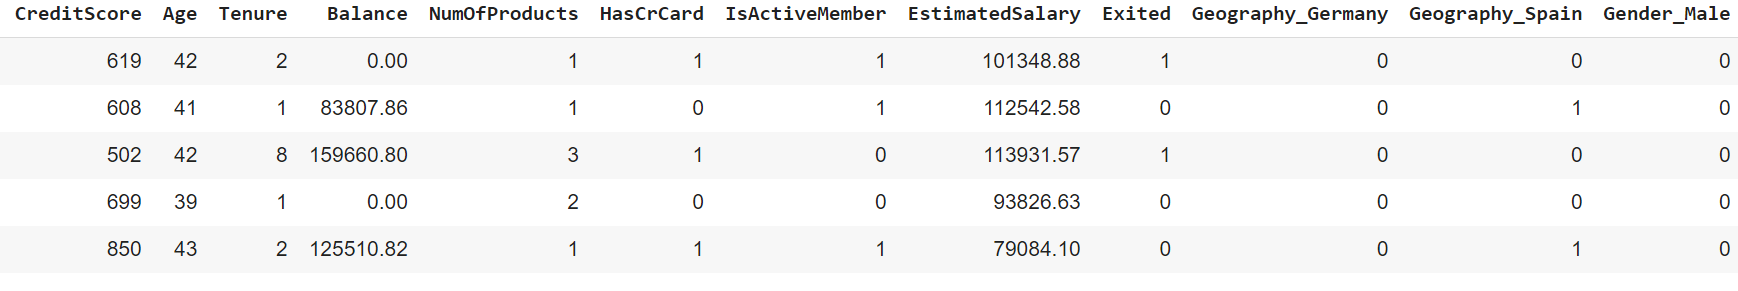
\includegraphics[width=1\textwidth]{Numerical.png}
    \caption{Standardization}
    \label{fig:enter-label}
\end{figure}

    
    \item Data Splitting: Before model building, we split the dataset into dependent (target) and independent (predictor) variables. This separation allows us to train the model on one portion of the data and evaluate its performance on another unseen portion.
\end{enumerate}

By effectively conducting data preparation, we can ensure that the data is ready for further analysis and model building. This will help us build an accurate and reliable customer churn prediction model, enabling the bank to proactively retain valuable customers and make data-driven decisions to improve customer satisfaction and loyalty.

\section{Exploratory Data Analysis}

Exploratory Data Analysis (EDA) is a critical phase in our customer churn prediction project that aims to gain deeper insights into the bank dataset and uncover meaningful patterns, relationships, and trends within the data. Through EDA, we explore and visualize the data to better understand its characteristics and potential factors that influence customer churn.

\subsection{Churn Analysis}

During the churn analysis, we focus on understanding the proportion of customers who have left the bank (churned) compared to those who have stayed. This analysis allows us to determine the churn rate, which is a fundamental metric for assessing customer retention performance. By identifying the churn rate, we can understand how many customers are leaving our business. This helps us measure the seriousness of the customer churn problem and its impact on our company's operations.

Additionally, our investigation into the relationship between customer churn and various independent variables (potential predictors) has enabled us to identify significant features that may influence customer churn. Understanding these predictors is vital for building an effective predictive model capable of accurately identifying customers at risk of churning. This model will empower the bank to take proactive measures and implement targeted retention strategies to improve overall customer satisfaction and reduce churn rates.

\subsection{Visualizing Customer Behavior}

Visualizations play a crucial role in our Exploratory Data Analysis (EDA), enabling us to understand complex relationships and patterns in the data. We have created various visual representations, such as count plots, pair plots, and hit map,  to explore the distribution of customer churn across different categories. One aspect we focused on is the churn count in relation to gender, allowing us to determine if gender plays a role in customer churn. Additionally, we examined churn patterns across different countries, providing valuable insights into potential regional variations in customer behavior.

Moreover, our analysis extended to other relevant features, such as age, account balance, customer tenure, credit score, estimated salary, number of products, etc... Visualizing these relationships has helped us uncover hidden patterns and draw actionable conclusions.

The outcomes of our exploratory data analysis will guide us in selecting the most relevant features to be used as independent variables in our predictive model. With a comprehensive understanding of the data, we can build a robust customer churn prediction model that will assist the bank in implementing targeted strategies to retain customers, reduce churn, and enhance overall customer satisfaction.

\section{Model Building}

Model Building is a crucial phase in our customer churn prediction project, where we develop a predictive model using machine learning algorithms to identify potential churners and make accurate predictions based on the dataset's features.

\subsection{Data Splitting and Standardization}

Before building the model, we splited the dataset into two parts: the training set and the testing set. The training set is used to train the machine learning model, while the testing set is used to evaluate the model's performance on unseen data.

Additionally, to ensure fair and effective model training, we standardized the data. Standardization involves scaling numerical features to have a mean of 0 and a standard deviation of 1. This step is essential for certain machine learning algorithms, as it prevents features with larger scales from dominating the model during training.

\subsection{Random Forest Classifier}

For this project, we will employed the Random Forest Classifier, a powerful ensemble learning algorithm. The Random Forest builds multiple decision trees during training and combines their predictions to make more accurate and robust predictions. This algorithm is particularly well-suited for classification tasks like customer churn prediction, as it can handle both numerical and categorical data and can capture complex relationships between features.

We trained the Random Forest Classifier on the training set, fine-tune its hyperparameters, and optimize its performance to achieve the best possible predictions.

\subsection{Model Evaluation Metrics}

After training the model, we evaluate its performance using various metrics to assess its predictive capabilities. Some of the key evaluation metrics we employ include: 

\begin{enumerate}
    \item Receiver Operating Characteristic (ROC) Curve: The ROC curve plots the true positive rate (sensitivity) against the false positive rate (1-specificity) at various classification thresholds. It provides a graphical representation of the model's ability to discriminate between churn and non-churn customers.

    \item Area Under the Curve (AUC) Score: The AUC score quantifies the overall performance of the model. A higher AUC score indicates better discrimination and model performance.
    
\begin{figure}[H]
    \centering
    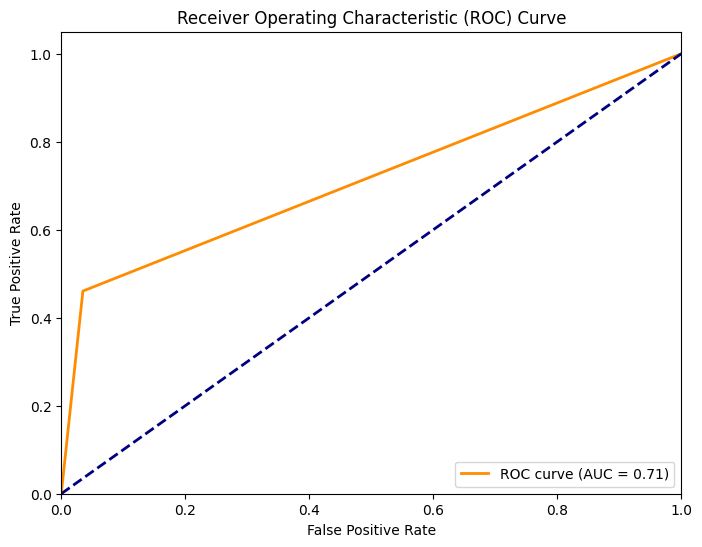
\includegraphics[width=0.8\textwidth]{ROC Curve.png}
\end{figure}


    \item Accuracy: The accuracy metric measures the proportion of correct predictions made by the model.
    \item Precision: Precision measures the proportion of true churners among the total predicted churners. It indicates the model's ability to avoid false positives.
    \item Recall (Sensitivity): Recall measures the proportion of actual churners correctly identified by the model. It indicates the model's ability to avoid false negatives.
    \item F1-score: The F1-score is the harmonic mean of precision and recall and provides a balanced evaluation of the model's performance.

           

\begin{figure}[H]
    \centering
    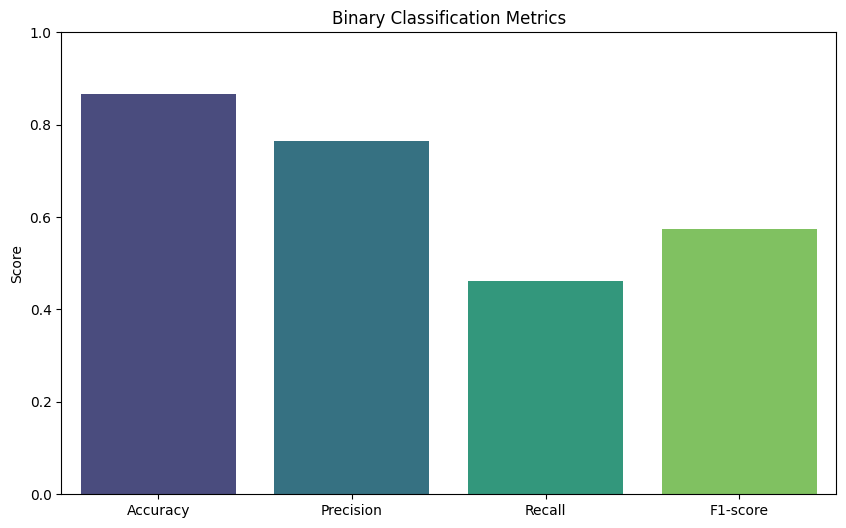
\includegraphics[width=1\textwidth]{Binary classification metrics.png}
\end{figure}


    \item Confusion Matrix: The Confusion Matrix is a table that presents the model's predictions, showing true positives (TP), true negatives (TN), false positives (FP), and false negatives (FN). It provides a comprehensive view of how well the model correctly classifies churn and non-churn instances.
\end{enumerate}


\begin{figure}[H]
    \centering
    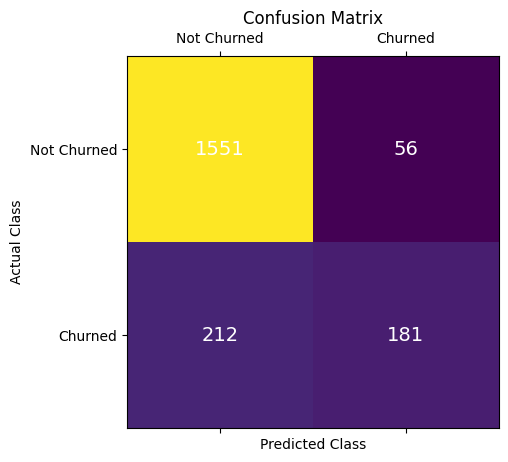
\includegraphics[width=1\textwidth]{Confusion matrix.png}
\end{figure}


The model building phase was a critical step in our customer churn prediction project. By using the Random Forest Classifier and evaluating its performance with various metrics, we aimed to create a reliable predictive model that can help the bank proactively retain customers and improve customer satisfaction.


\section{Conclusion}

In conclusion, we successfully developed a customer churn prediction model for the bank dataset using the Random Forest Classifier. Through data preparation and exploratory data analysis, we gained valuable insights into customer behavior and identified potential factors influencing churn. The model's evaluation metrics, such as ROC curve, AUC score, accuracy, precision, recall, and F1-score, demonstrated its effectiveness in predicting customer churn. Armed with this predictive model, the bank can proactively retain customers, improve customer satisfaction, and optimize its services for better business outcomes.
In our collaborative project, each team member played a vital role in contributing their effort to achieve our objectives. 

Group Organization:

Google Colaboratory: Ezginur Cendik

LaTex Document Writer: Mustafa Kemal Kaya

GitHub: Ezginur Cendik, Mustafa Kemal Kaya


\bibliographystyle{plain}
\bibliography{mybib}
\end{document}
